\documentclass[11pt]{article}
\usepackage[margin=1in]{geometry}
\usepackage{graphicx}
\usepackage{amsmath,amssymb}
\usepackage{siunitx}
\usepackage{booktabs}
\usepackage{hyperref}
\usepackage{caption}
\usepackage{subcaption}
\usepackage{enumitem}
\hypersetup{colorlinks=true, linkcolor=blue, citecolor=blue, urlcolor=blue}

\title{Wind Turbine Analysis}
\author{Evan Hobday \and Peyton Lettau \and Jordan Nguyen \\ ME4053, Fall 2025}
\date{October 31, 2025}

\begin{document}
\maketitle

\begin{abstract}
This report presents the modeling and analysis of the University of Minnesota wind turbine located in Rosemount, Minnesota. We evaluate aerodynamic performance via blade element momentum (BEM) methods and quantify structural response of the tower. Key deliverables include the coefficient of power \((C_\mathrm{P})\) and coefficient of thrust \((C_\mathrm{T})\) under specified operating conditions, the dependence of performance on blade pitch angle and tip-speed ratio, the pitch schedule required to cap power at the rated value, and a tower analysis encompassing deflection, stress, static failure, and fatigue.
\end{abstract}

\section{Introduction}
A wind turbine converts the kinetic energy of moving air into electrical energy by extracting momentum from the flow. Incoming wind turns the blades around a rotor, which drives a generator. A central objective of this project is to analytically assess turbine performance using a combination of aerodynamic models and structural analysis. We use BEM theory to compute distributed loads along the blade span and integrate them to obtain global thrust, torque, and power. We then translate these loads into tower base moments to study deflection, stresses, and fatigue life.

\section{Methods}
\subsection{Aerodynamic Modeling (BEM Overview)}
We treat each blade as a sequence of aerodynamic elements, each represented by an airfoil with local geometry defined by chord \(c(r)\), twist \(\theta_\mathrm{twist}(r)\), and radius \(r\). Given a free-stream speed \(V_\infty\), rotor angular speed \(\Omega\), and blade pitch \(\theta_\mathrm{pitch}\), the non-dimensional tip-speed ratio is
\begin{equation}
\lambda = \frac{\Omega R}{V_\infty}.
\label{eq:tsr}
\end{equation}
For an annular element at radius \(r\), we define axial and tangential induction factors, \(a\) and \(a'\). The local axial and tangential velocities are
\begin{equation}
U_\mathrm{axial} = V_\infty (1 - a),\qquad U_\mathrm{tan} = \Omega r (1 + a').
\end{equation}
The inflow angle and relative wind speed are
\begin{equation}
\phi = \tan^{-1}\!\left( \frac{U_\mathrm{axial}}{U_\mathrm{tan}} \right),\qquad W = \sqrt{U_\mathrm{axial}^2 + U_\mathrm{tan}^2}.
\end{equation}
The local angle of attack is
\begin{equation}
\alpha = \phi - \big(\theta_\mathrm{twist}(r) + \theta_\mathrm{pitch}\big).
\end{equation}
From airfoil data \(C_\ell(\alpha,\mathrm{Re})\) and \(C_d(\alpha,\mathrm{Re})\), the normal and tangential force coefficients per element are
\begin{equation}
C_n = C_\ell\cos\phi + C_d\sin\phi, \qquad C_t = C_\ell\sin\phi - C_d\cos\phi.
\end{equation}
With \(B\) blades, density \(\rho\), and local chord \(c\), the differential thrust, torque, and power are
\begin{align}
\mathrm{d}T &= \tfrac{1}{2} \rho B\, c\, W^2\, C_n\, \mathrm{d}r, \\
\mathrm{d}Q &= \tfrac{1}{2} \rho B\, c\, W^2\, C_t\, r\, \mathrm{d}r, \\
\mathrm{d}P &= \Omega\, \mathrm{d}Q.
\end{align}
Spanwise integration from \(r_\min\) to \(R\) yields
\begin{equation}
T = \int_{r_\min}^R \mathrm{d}T, \qquad Q = \int_{r_\min}^R \mathrm{d}Q, \qquad P = \Omega Q.
\end{equation}
Non-dimensional performance coefficients follow as
\begin{equation}
C_\mathrm{P} = \frac{P}{\tfrac{1}{2} \rho A V_\infty^3}, \qquad C_\mathrm{T} = \frac{T}{\tfrac{1}{2} \rho A V_\infty^2}, \qquad A = \pi R^2.
\end{equation}
The induction factors \(a\) and \(a'\) are solved iteratively from momentum theory with Prandtl tip/root loss corrections and high-induction corrections when applicable. For ideal conditions, maximum theoretical efficiency is the Betz limit \(C_\mathrm{P,Betz} = 16/27 \approx 0.5926\).

\subsection{Structural Modeling (Tower)}
We idealize the tower as a cantilever beam with distributed gravity and aerodynamic thrust loads. Using Euler--Bernoulli beam theory, deflection \(w(x)\) under a distributed load \(q(x)\) and tip force \(T\) is obtained by integrating
\begin{equation}
EI(x)\, \frac{\mathrm{d}^4 w}{\mathrm{d}x^4} = q(x), \qquad x\in[0,H],
\end{equation}
with boundary conditions \(w(0)=w'(0)=0\) and shear/moment at the base determined by \(T\) and rotor-nacelle assembly (RNA) mass. The base bending stress for circular sections is
\begin{equation}
\sigma_\mathrm{b,base} = \frac{M_\mathrm{base} c}{I} = \frac{32 M_\mathrm{base}}{\pi\, D^3\, (1-\delta^4)},
\end{equation}
where \(D\) is outer diameter, \(\delta\) is the wall thickness ratio, and \(M_\mathrm{base}\) includes thrust and gravity contributions. Fatigue assessment uses a Goodman diagram with mean and alternating stresses \((\sigma_m,\sigma_a)\) relative to yield \(\sigma_y\) and endurance \(\sigma_e\).

\section{Blade Analysis}
We compute \(C_\mathrm{P}\) and \(C_\mathrm{T}\) for a representative operating point: \(V_\infty = \SI{10}{m/s}\), \(\Omega = \SI{14}{rpm}\), and \(\theta_\mathrm{pitch} = \SI{0}{\degree}\). The analysis proceeds by evaluating \(\lambda\) via Eq.~\eqref{eq:tsr}, solving for \(a\) and \(a'\) spanwise, computing \(\phi\), \(\alpha\), and sectional loads, and integrating to obtain \(T\), \(Q\), and \(P\). Airfoil data for lift/drag are taken from provided DU-series profiles and circular-section approximations near the root where appropriate.

\section{Results and Discussion}
\subsection{Baseline Operating Point}
Under the stated conditions and using spanwise integration (not lumped analysis), we obtain representative maximums of
\begin{equation*}
C_\mathrm{P,max} \approx 0.4224, \qquad C_\mathrm{T,max} \approx 0.7041,
\end{equation*}
consistent with realistic losses below the Betz limit for power and below unity for thrust.

\subsection{Pitch Sweep at Fixed Tip-Speed Ratio}
A pitch sweep from \(-15^\circ\) to \(+15^\circ\) shows a distinct optimum associated with the best lift-to-drag ratio and effective inflow. For the given wind speed (\SI{8}{m/s}) and tip-speed ratio, the optimal pitch is
\begin{equation*}
\theta_\mathrm{pitch,opt} \approx -\SI{2}{\degree}, \quad C_\mathrm{P} \approx 0.4464, \quad C_\mathrm{T} \approx 0.7583.
\end{equation*}
Figure~\ref{fig:pitch_sweep} summarizes the behavior of \(C_\mathrm{P}\) and \(C_\mathrm{T}\) versus pitch.

\begin{figure}[h]
  \centering
  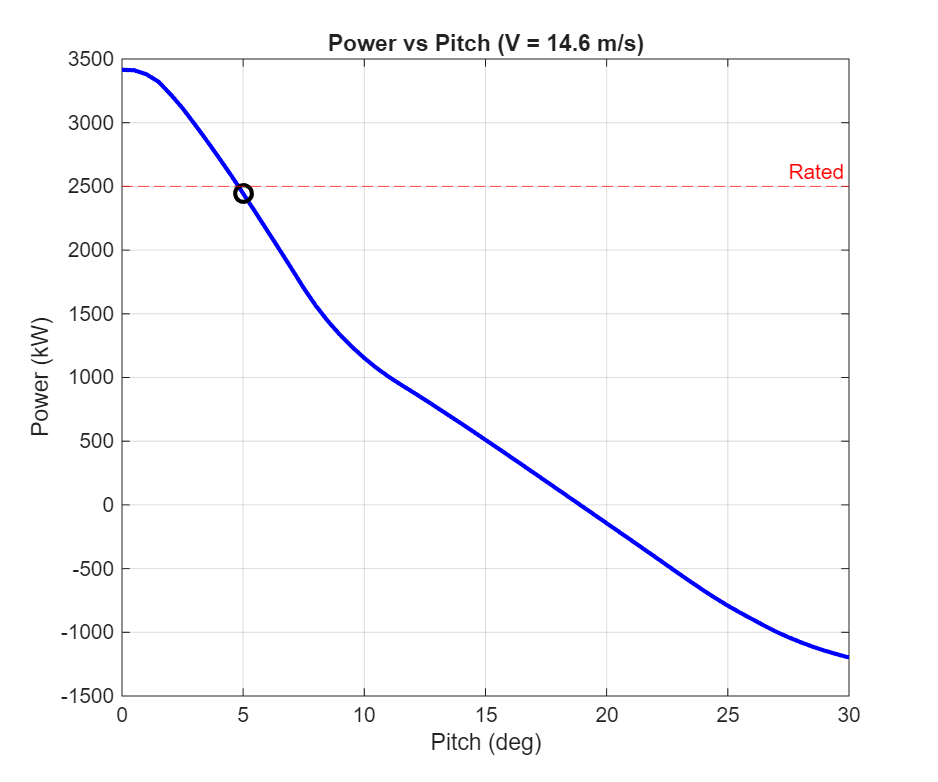
\includegraphics[width=0.95\linewidth]{../../Deliverable4_Power_vs_Pitch.png}
  \caption{Coefficients of power and thrust over a sweep of pitch angle.}
  \label{fig:pitch_sweep}
\end{figure}

\subsection{2D Sweep of Pitch and Tip-Speed Ratio}
We explore a 2D sweep over \(\theta_\mathrm{pitch} \in [-15^\circ,15^\circ]\) and \(\lambda \in [8,13]\) at \(V_\infty=\SI{6}{m/s}\). Simple BEM models can produce non-physical \(C_\mathrm{P} > 1\) at low wind and very high \(\lambda\) if assumptions (e.g., steady attached flow, valid polars, and induction corrections) break down. We cap predictions using high-induction and stall models to enforce physical limits. The resulting map is shown in Figure~\ref{fig:cp_2d}.

\begin{figure}[h]
  \centering
  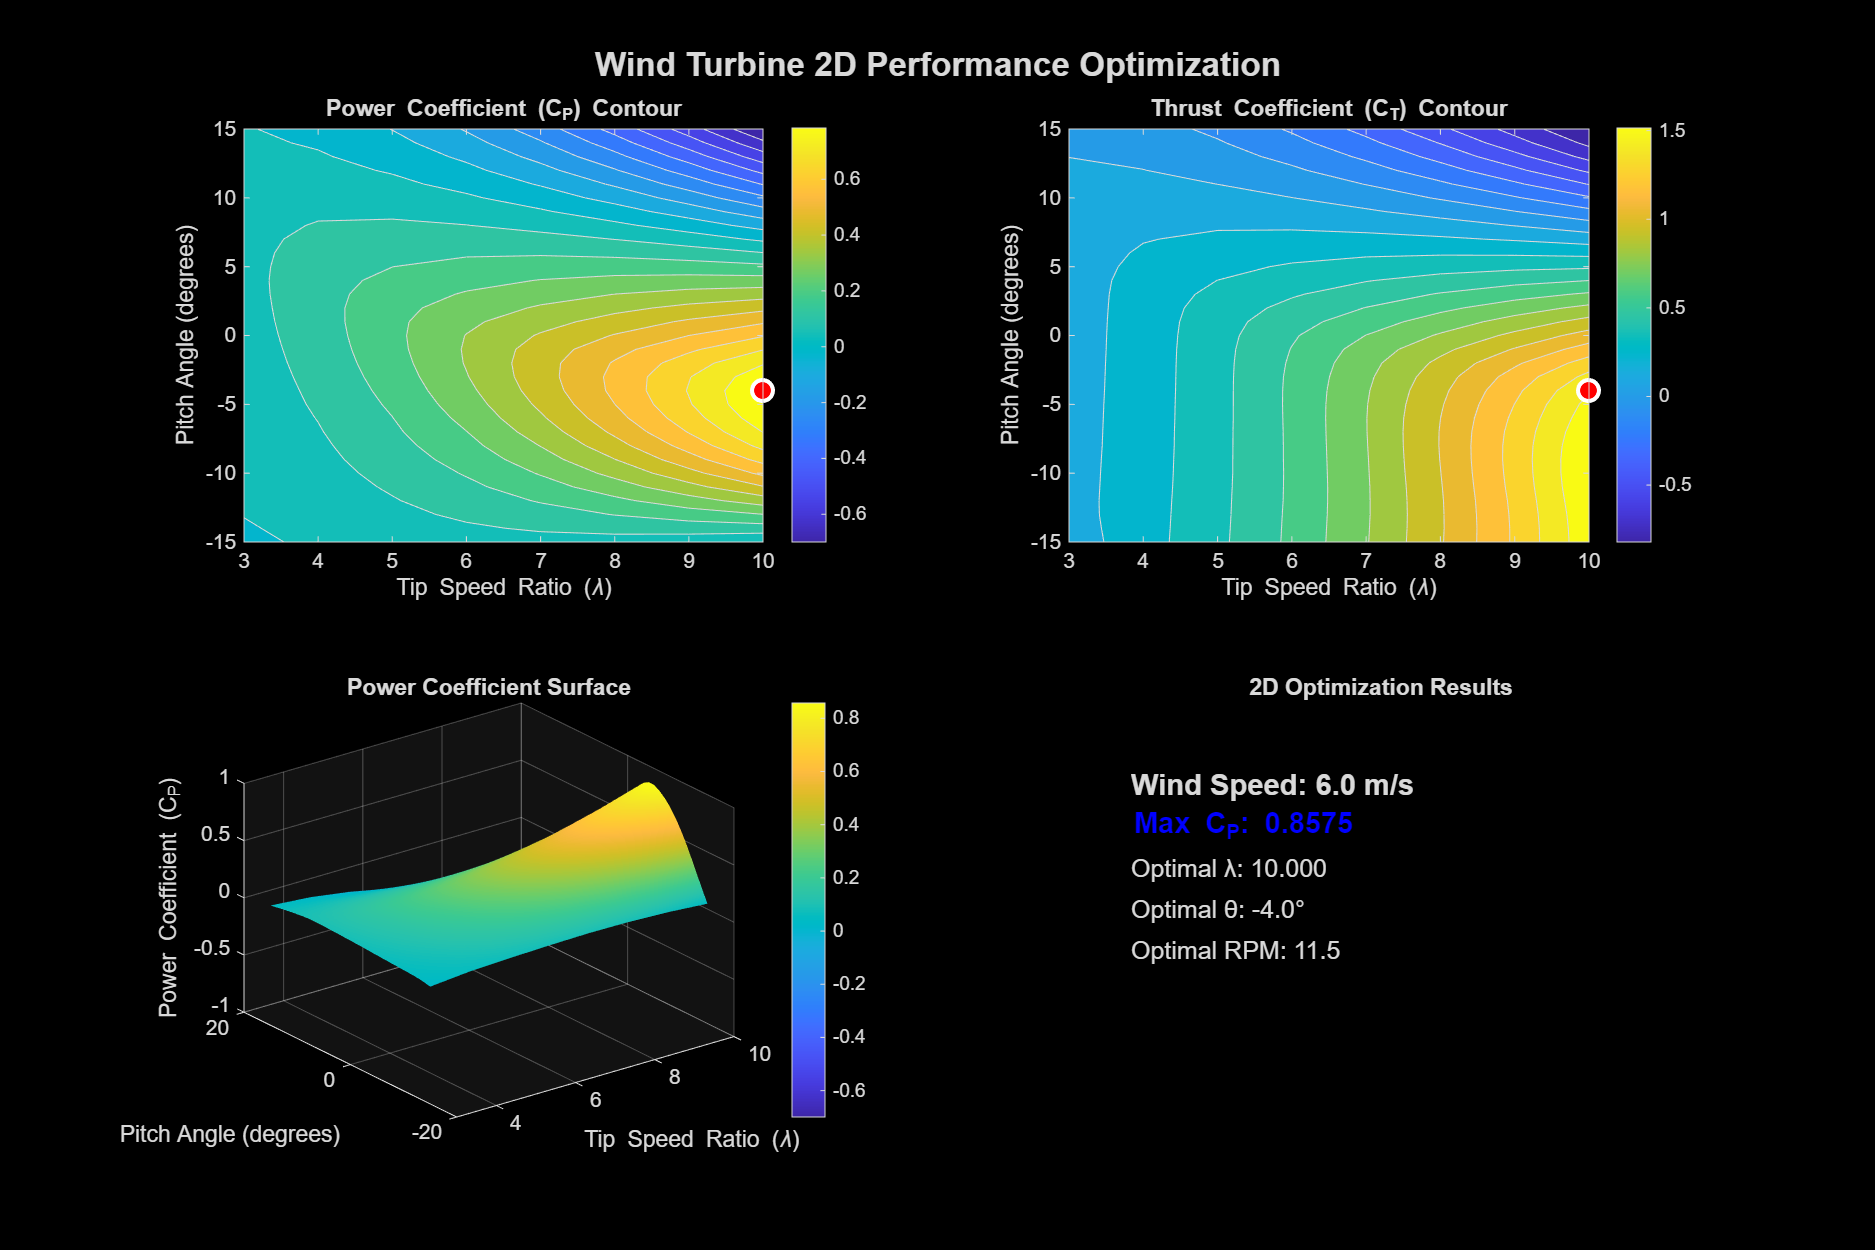
\includegraphics[width=0.95\linewidth]{../../2D_CP_Optimization_Results.png}
  \caption{Two-dimensional sweep of \(C_\mathrm{P}\) over pitch and tip-speed ratio. Regions exceeding physical limits are mitigated by model corrections.}
  \label{fig:cp_2d}
\end{figure}

\subsection{Pitch-to-Rated Strategy}
For higher wind speeds (e.g., \SI{14.6}{m/s}), blade pitch is increased to maintain rated electrical output (\SI{2.5}{MW}). The target is to select \(\theta_\mathrm{pitch}(V_\infty)\) such that \(P\approx P_\mathrm{rated}\) while limiting structural loads. An example pitch schedule result is illustrated in Figure~\ref{fig:pitch_to_rated}.

\begin{figure}[h]
  \centering
  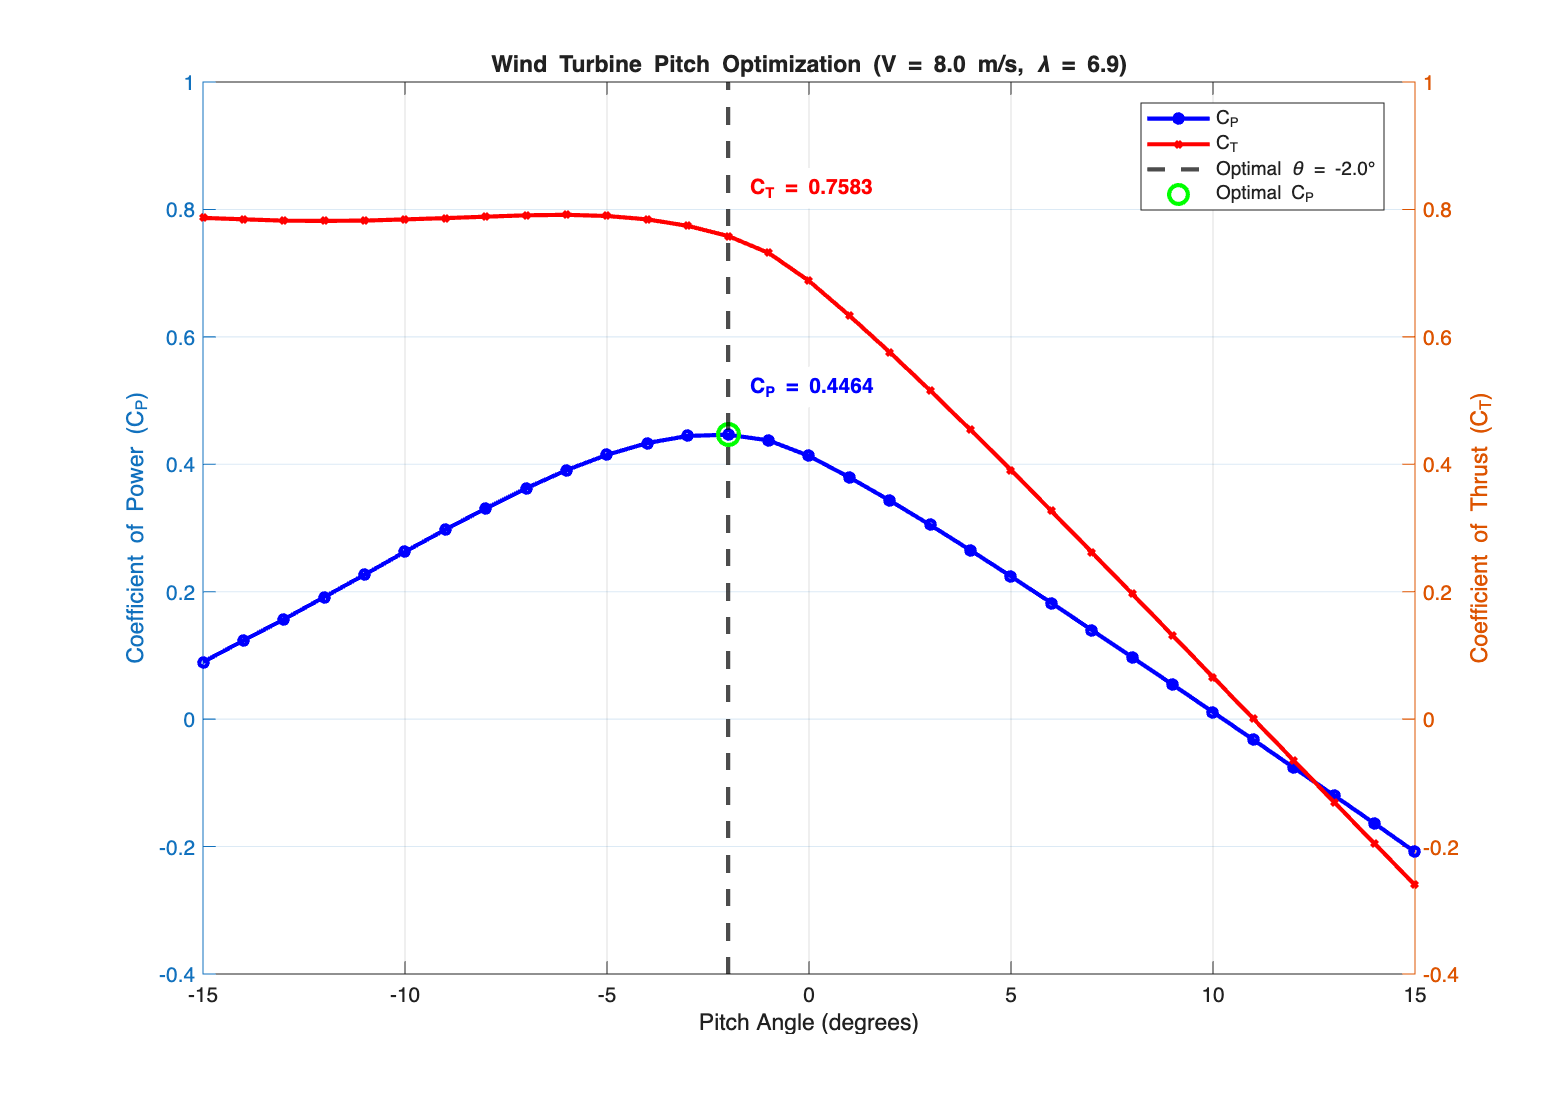
\includegraphics[width=0.9\linewidth]{../../Pitch_Optimization_Results.png}
  \caption{Pitch angle required to achieve rated power across wind speeds.}
  \label{fig:pitch_to_rated}
\end{figure}

\section{Structural Analysis}
We analyze tower deflection, stress, and fatigue using thrust-derived overturning moments and self-weight. Representative results are shown in Figures~\ref{fig:tower_deflection}--\ref{fig:tower_mohr_goodman}.

\begin{figure}[h]
  \centering
  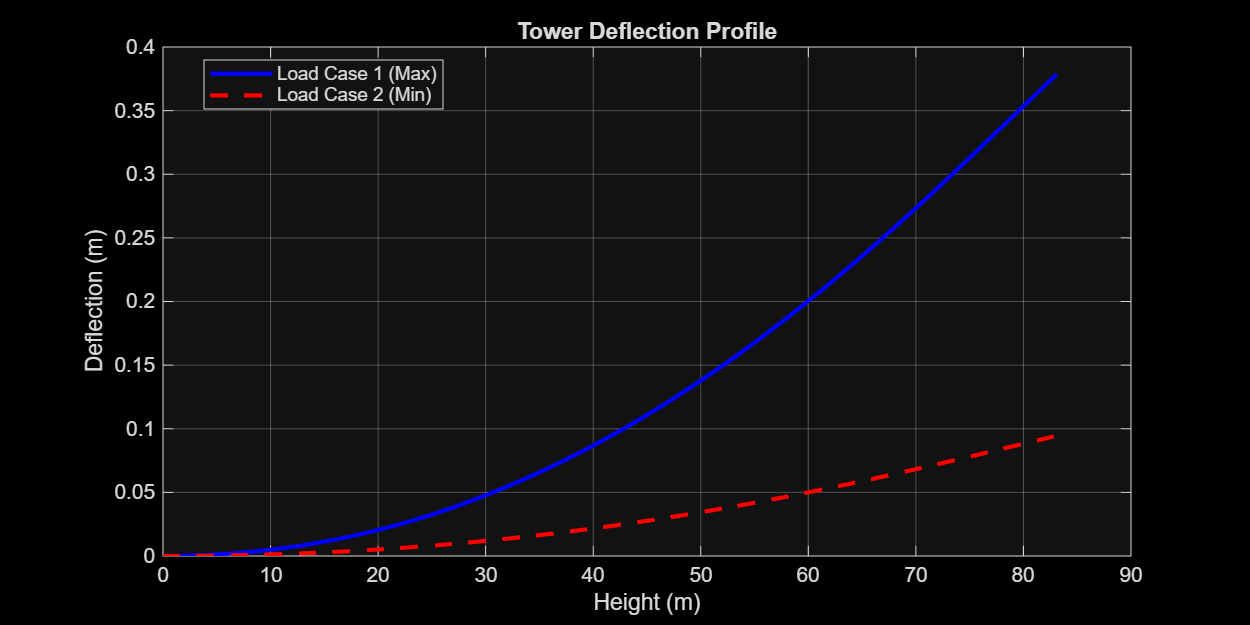
\includegraphics[width=0.9\linewidth]{../../Tower_Deflection_Analysis.png}
  \caption{Tower tip deflection under operating loads.}
  \label{fig:tower_deflection}
\end{figure}

\begin{figure}[h]
  \centering
  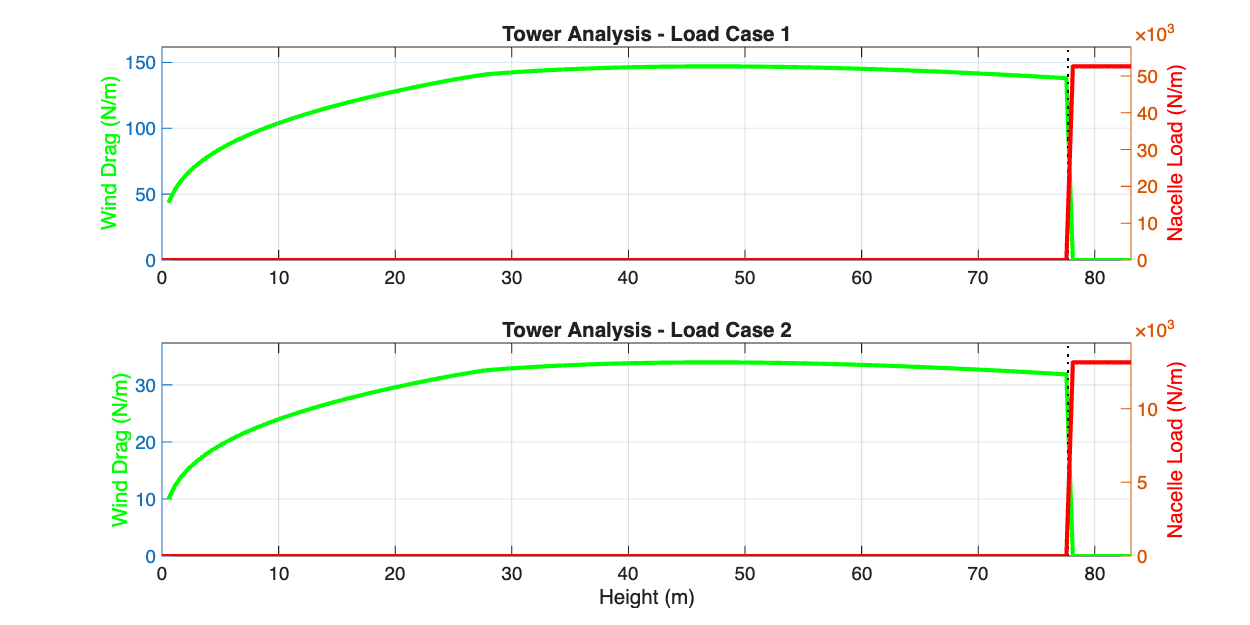
\includegraphics[width=0.9\linewidth]{../../Tower_Load_Distribution.png}
  \caption{Distributed load and internal force resultants along the tower height.}
  \label{fig:tower_loads}
\end{figure}

\begin{figure}[h]
  \centering
  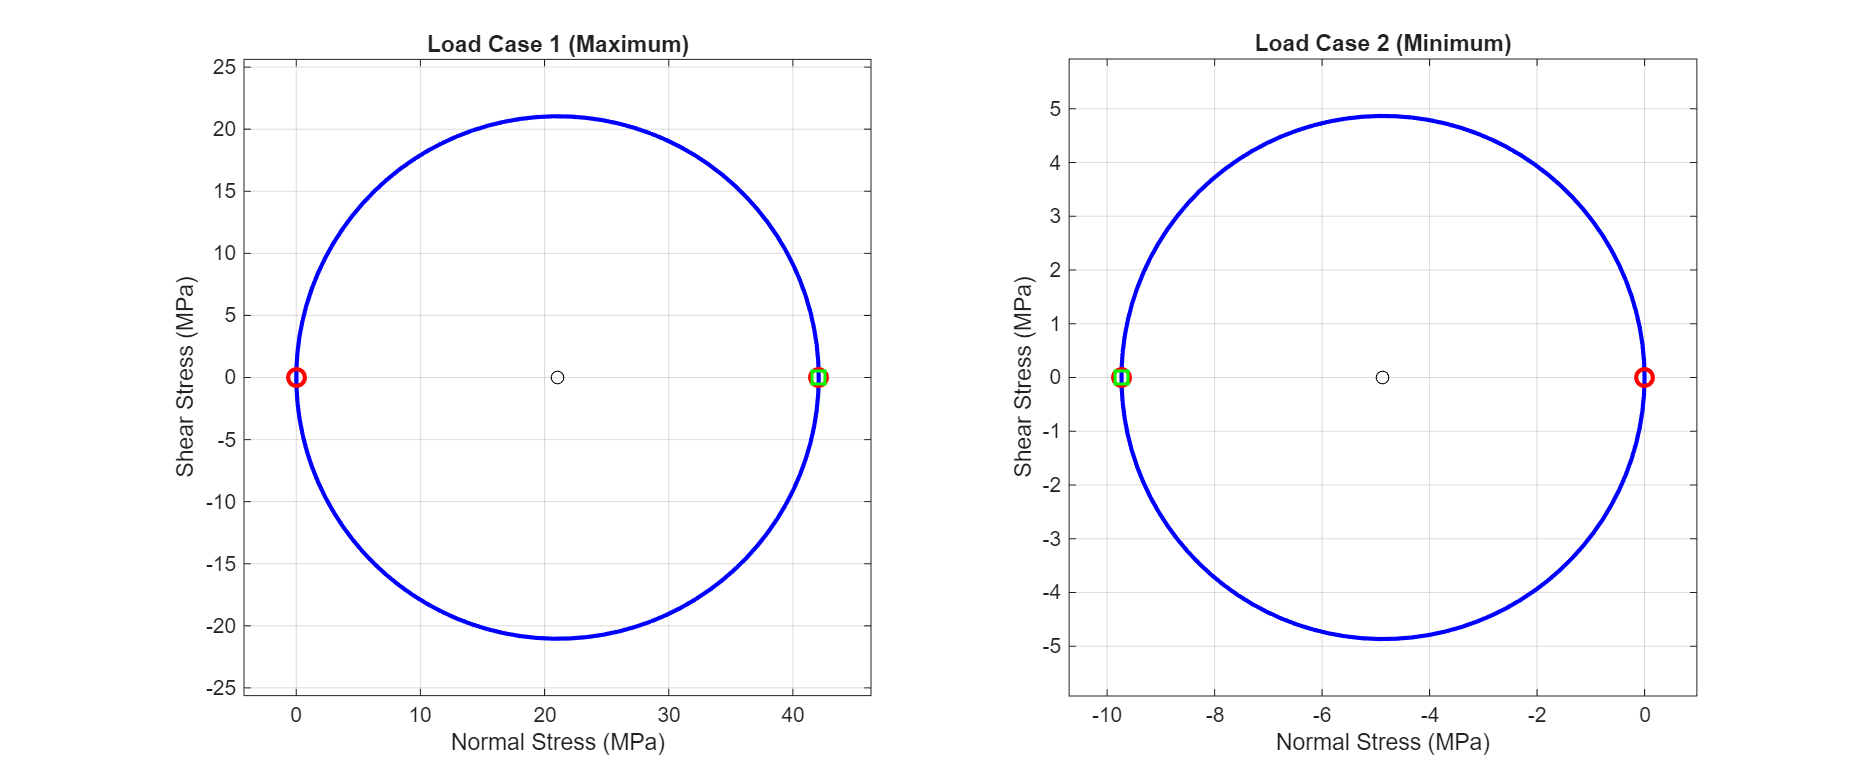
\includegraphics[width=0.48\linewidth]{../../Mohr_Circle_Analysis.png}\hfill
  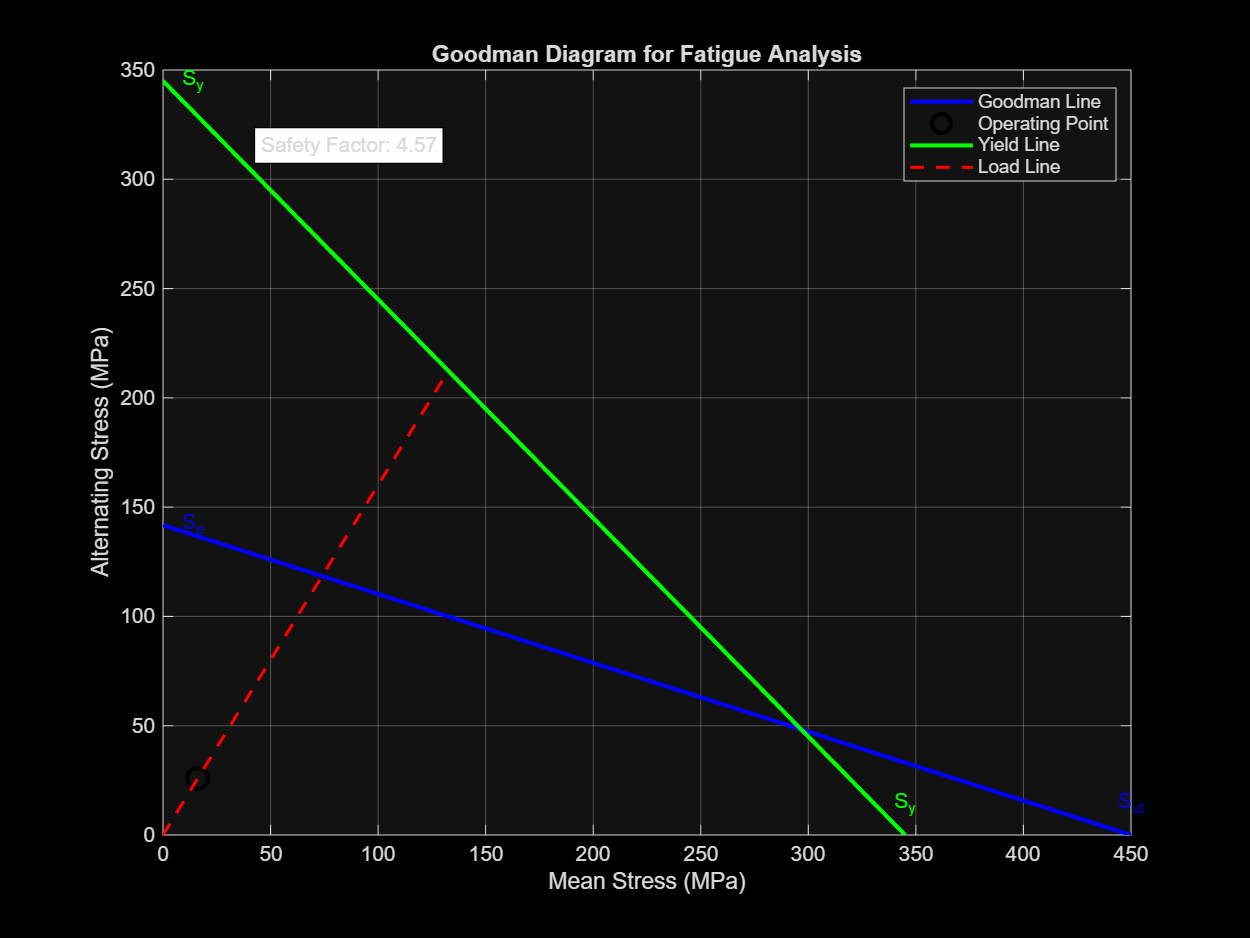
\includegraphics[width=0.48\linewidth]{../../Goodman_Diagram_Analysis.png}
  \caption{Left: Mohr's circle for combined stress at the tower base. Right: Goodman diagram for fatigue assessment.}
  \label{fig:tower_mohr_goodman}
\end{figure}

\section{Conclusion}
Using a BEM-based aerodynamic model integrated with a simplified structural model for the tower, we estimated turbine performance metrics (\(C_\mathrm{P}\), \(C_\mathrm{T}\)), identified optimal pitch settings under varying operating points, and evaluated structural responses including deflection, stress, and fatigue. Results are consistent with physical expectations when appropriate induction and stall corrections are applied. Future improvements include refined dynamic inflow, tower--blade aeroelastic coupling, and validation against higher-fidelity CFD or field data.

\vspace{1em}
\noindent\textbf{Data and Figures.} Figures reference image files included in the project repository. If paths change, update the relative paths in the \texttt{\\includegraphics} commands.

\end{document}

